\subsection{Fase 1 (2018-12-04 - 2019-01-21)}
	\subsubsection{Ore impiegate}
	La seguente tabella indica le ore impiegate durante la fase 1. Tra parentesi viene indicata la differenza tra ore preventivate e ore impiegate ($preventivo - consuntivo$): valori positivi indicano le ore risparmiate e valori negativi indicano le ore in eccesso.
	
	\begin{table}[H]
		\centering
		\begin{tabular}{| l | c c c c c c | c |}
			\rowcolor{LightBlue}
			& \multicolumn{7}{c}{\textbf{\color{white}Numero di ore}}	\\	
			\rowcolor{LightBlue}
			\textbf{\color{white}Membro}
			& \textbf{\color{white}RES}
			& \textbf{\color{white}AMM}
			& \textbf{\color{white}AN}
			& \textbf{\color{white}PRO}
			& \textbf{\color{white}DEV}
			& \textbf{\color{white}VER}
			& \textbf{\color{white}Totali}\\	
			Bergo     		& -  (0)		& 9  (+6) 	& 22 (-8) 		& - (0) & - (0) & 7  (+1) 	& 38\\
			Bortone   		& -  (0)		& 14 (-4) 	& 18 (-3) 		& - (0) & - (0) & 10 (-2)	& 42\\
			Cosentino 		& 25 (-5) 	& -  (0) 	& 24 (-2) 		& - (0) & - (0) & -  (+5)	& 49\\
			Marcato   		& 10 (-5) 	& 10 (0) 	& 22 (+3) 		& - (0) & - (0) & -  (+3)	& 42\\
			Peagno    		& -  (+5) 	& 15 (0) 	& 23 (-1) 		& - (0) & - (0) & -  (+3)	& 38\\
			Peron     		& -  (0)		& 13 (-3) 	& 23 (+6) 		& - (0) & - (0) & 13 (-8)	& 49\\
			Pettenuzzo 	& - (0) 		& 12 (+3) 	& 5  (+14) 	& - (0) & - (0) & 13 (-8)	& 30\\ \hline
		\end{tabular}
		\caption{Ore di lavoro impiegate per membro/ruolo della fase 1}
	\end{table}
	
	\begin{figure}[H]
		\centering
		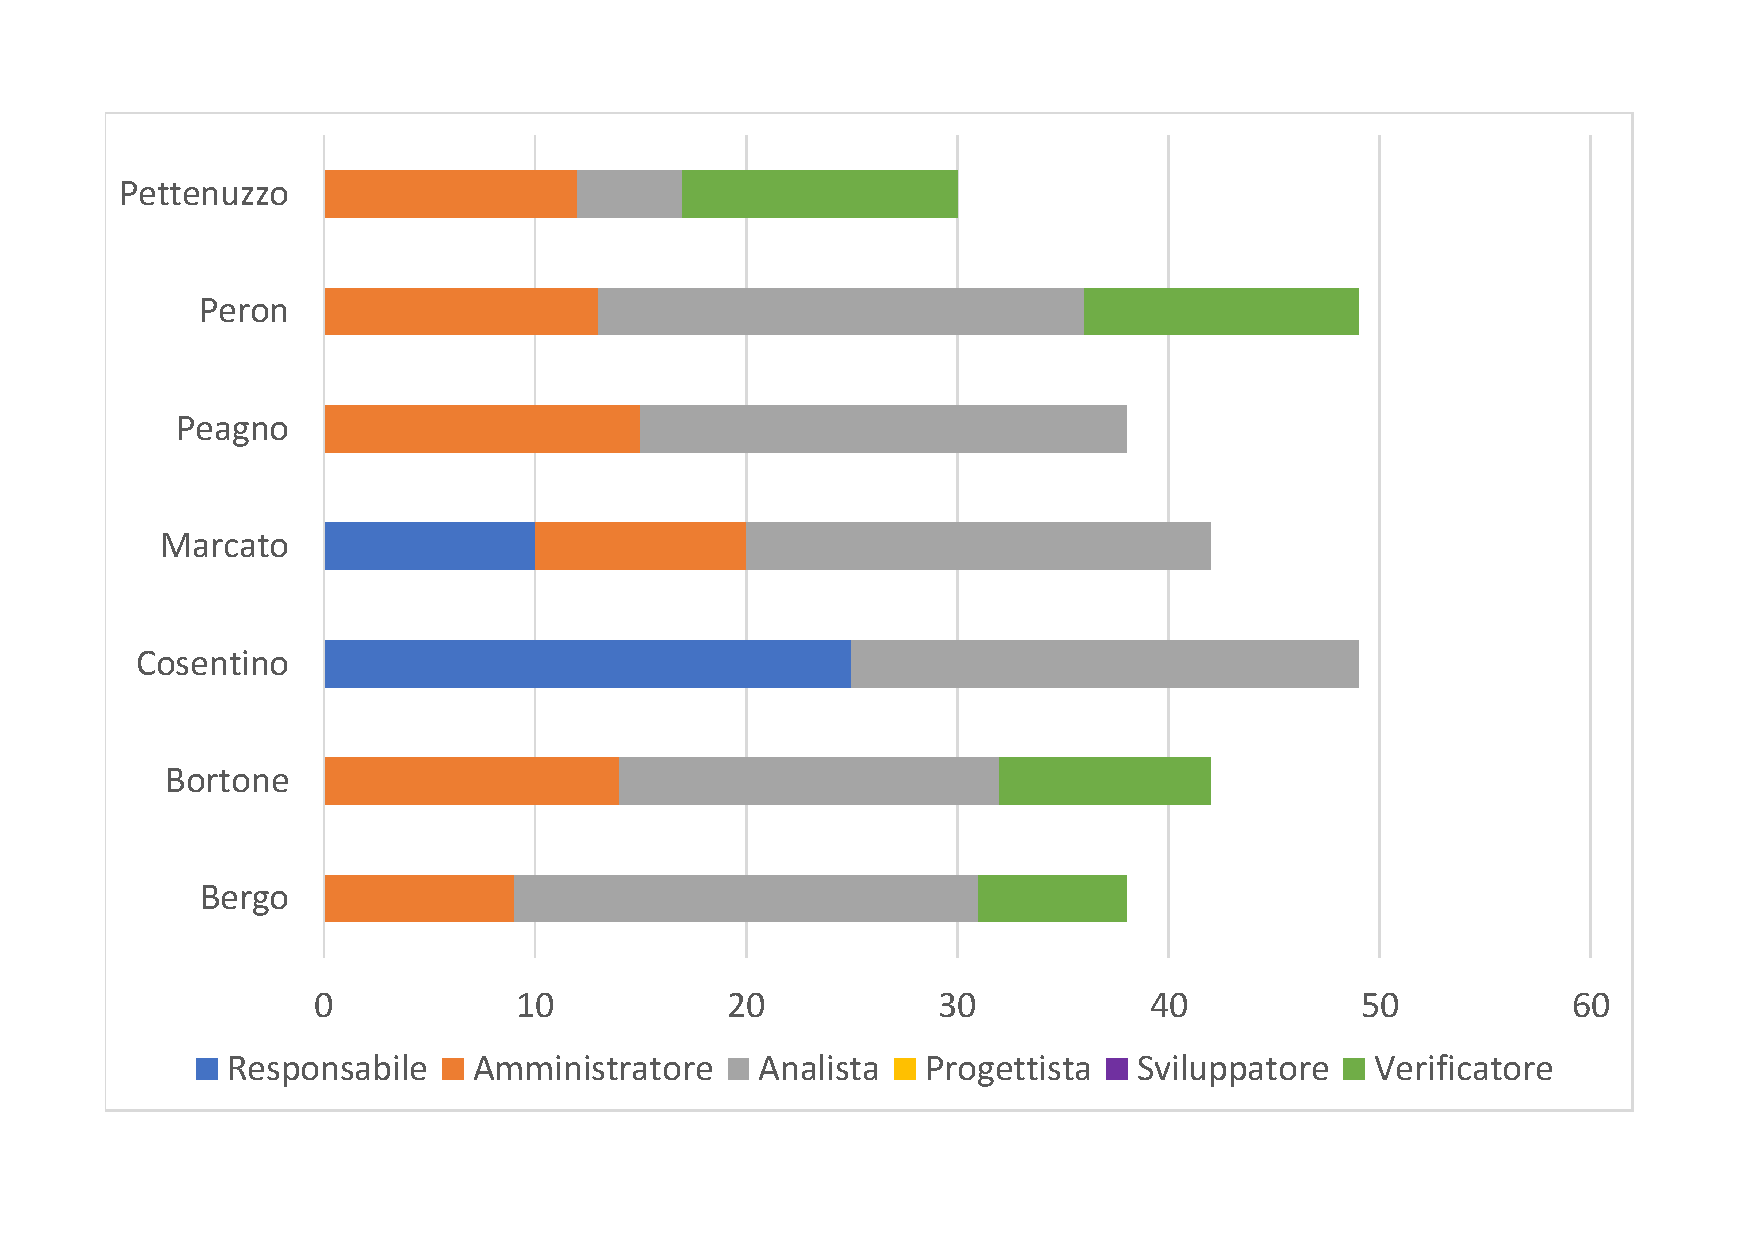
\includegraphics[scale=0.45]{images/consuntivoRR.pdf}
		\caption{Istogramma del consuntivo della fase 1}
	\end{figure}
	
	\subsubsection{Costo}
	Le seguenti tabelle indicano i costi della fase 1. Nell'ultima colonna vengono indicate le differenze tra costi previsti e costi effettivi ($previsto - effettivo$): valori positivi indicano i risparmi e valori negativi indicano le perdite.
	
	\begin{table}[H]
		\centering
		\begin{tabular}{| l | l | l |}
			\rowcolor{LightBlue}
			\textbf{\color{white}Membro}
			& \textbf{\color{white}Costo}
			& \textbf{\color{white}Differenza}\\			
			Bergo 				& 835€ 	& -65€\\
			Bortone 			& 880€ 	& -185€\\
			Cosentino 		& 1350€ 	& -125€\\
			Marcato 			& 1050€ 	& -30€\\
			Peagno 			& 875€ 	& +170€\\
			Peron 				& 1030€ 	& -30€\\
			Pettenuzzo 	& 560€ 	& +290€\\ \hline
			\textbf{Totale} & 6580€ & +25€\\ \hline
		\end{tabular}
		\caption{Costo effettivo di ciascun membro nella fase 1}	
	\end{table}

	\begin{table}[H]
		\centering
		\begin{tabular}{| l | l |l|}
			\rowcolor{LightBlue}
			\textbf{\color{white}Membro}
			& \textbf{\color{white}Costo}
			& \textbf{\color{white}Differenza}\\
			Responsabile 		& 1050€ 	& -150€\\
			Amministratore 	& 1460€ 	& +40€\\
			Analista 				& 3425€ 	& +225€\\
			Progettista 			& 0€ 		& 0€\\
			Programmatore 		& 0€ 		& 0€\\
			Verificatore 		& 645€ 	& -90€\\ \hline
			\textbf{Totale} 	& 6580€ 	& +25€\\ \hline
		\end{tabular}
		\caption{Costo effettivo di ciascun ruolo nella fase 1}
	\end{table}

	\subsubsection{Conclusioni}
		\paragraph{Costi\\}
La cifra prevista per l'investimento era di \textbf{6605€} e vi è stato un risparmio di \textbf{25€}. I costi effettivi ammontano, quindi, a \textbf{6580€}. 
		\paragraph{Scostamenti\\}
Vi sono stati dei leggeri scostamenti rispetto a quanto previsto. Ciò è imputabile a una previsione troppo pessimista delle ore necessarie per ogni attività. Tuttavia, un altro motivo può essere individuato nel mancato rispetto delle assegnazioni delle attività. Ciò è stato causato dalla frenesia da cui si è fatto prendere il gruppo nella parte successiva al periodo natalizio. Infatti, tra il 2018-12-21 e il 2019-01-06 i tempi non sono stati rispettati a causa di problemi di comunicazione tra i membri del gruppo. In seguito, a queste considerazioni è stato aggiunto alla tabella in §2.1 il rischio G03.

\newpage	
\subsection{Fase 2 (2019-01-22 - 2019-03-15)}
	\subsubsection{Ore impiegate}
La seguente tabella indica le ore impiegate durante la fase 2. Tra parentesi viene indicata la differenza tra ore preventivate e ore impiegate ($preventivo - consuntivo$): valori positivi indicano le ore risparmiate e valori negativi indicano le ore in eccesso.

		\begin{table}[H]
			\centering
		\begin{tabular}{| l | c c c c c c | c |}
			\rowcolor{LightBlue}
			& \multicolumn{7}{c}{\textbf{\color{white}Numero di ore}}	\\
	
			\rowcolor{LightBlue}
			\textbf{\color{white}Membro}
			& \textbf{\color{white}RES}
			& \textbf{\color{white}AMM}
			& \textbf{\color{white}AN}
			& \textbf{\color{white}PRO}
			& \textbf{\color{white}DEV}
			& \textbf{\color{white}VER}
			& \textbf{\color{white}Totali}\\
			Bergo     		& -  (0)		& 5  (0) 	& -  (0) 		& 18 (-3) & 10 (0) & 5  (0) 	& 38\\
			Bortone   		& -  (0)		& -  (0) 	& -  (0) 		& 22 (-1) & 9 (0) & -  (0)	& 31\\
			Cosentino 		& -  (0)	 	& -  (0) 	& 7  (-2) 		& 15 (-2) & 5 (0) & 5  (0)	& 32\\
			Marcato   		& -  (0) 		& 10  (0) 	& -  (0) 		& 10 (0) & 7 (0) & 5  (0)	& 32\\
			Peagno    		& -  (0) 		& 8  (0) 	& -  (0) 		& 10 (6) & - (0) & 10  (0)	& 28\\
			Peron     		& 15  (0)		& -  (0) 	& -  (0) 		& 13 (-3) & 10 (0) & -  (0)	& 38\\
			Pettenuzzo 		& 15  (0) 		& -  (0) 	& 8  (2) 		& 7 (-2) & - (0) & -  (0)	& 30\\ \hline
		\end{tabular}
		\caption{Ore di lavoro impiegate per membro/ruolo della fase 2}
	\end{table}
	
	\begin{figure}[H]
		\centering
		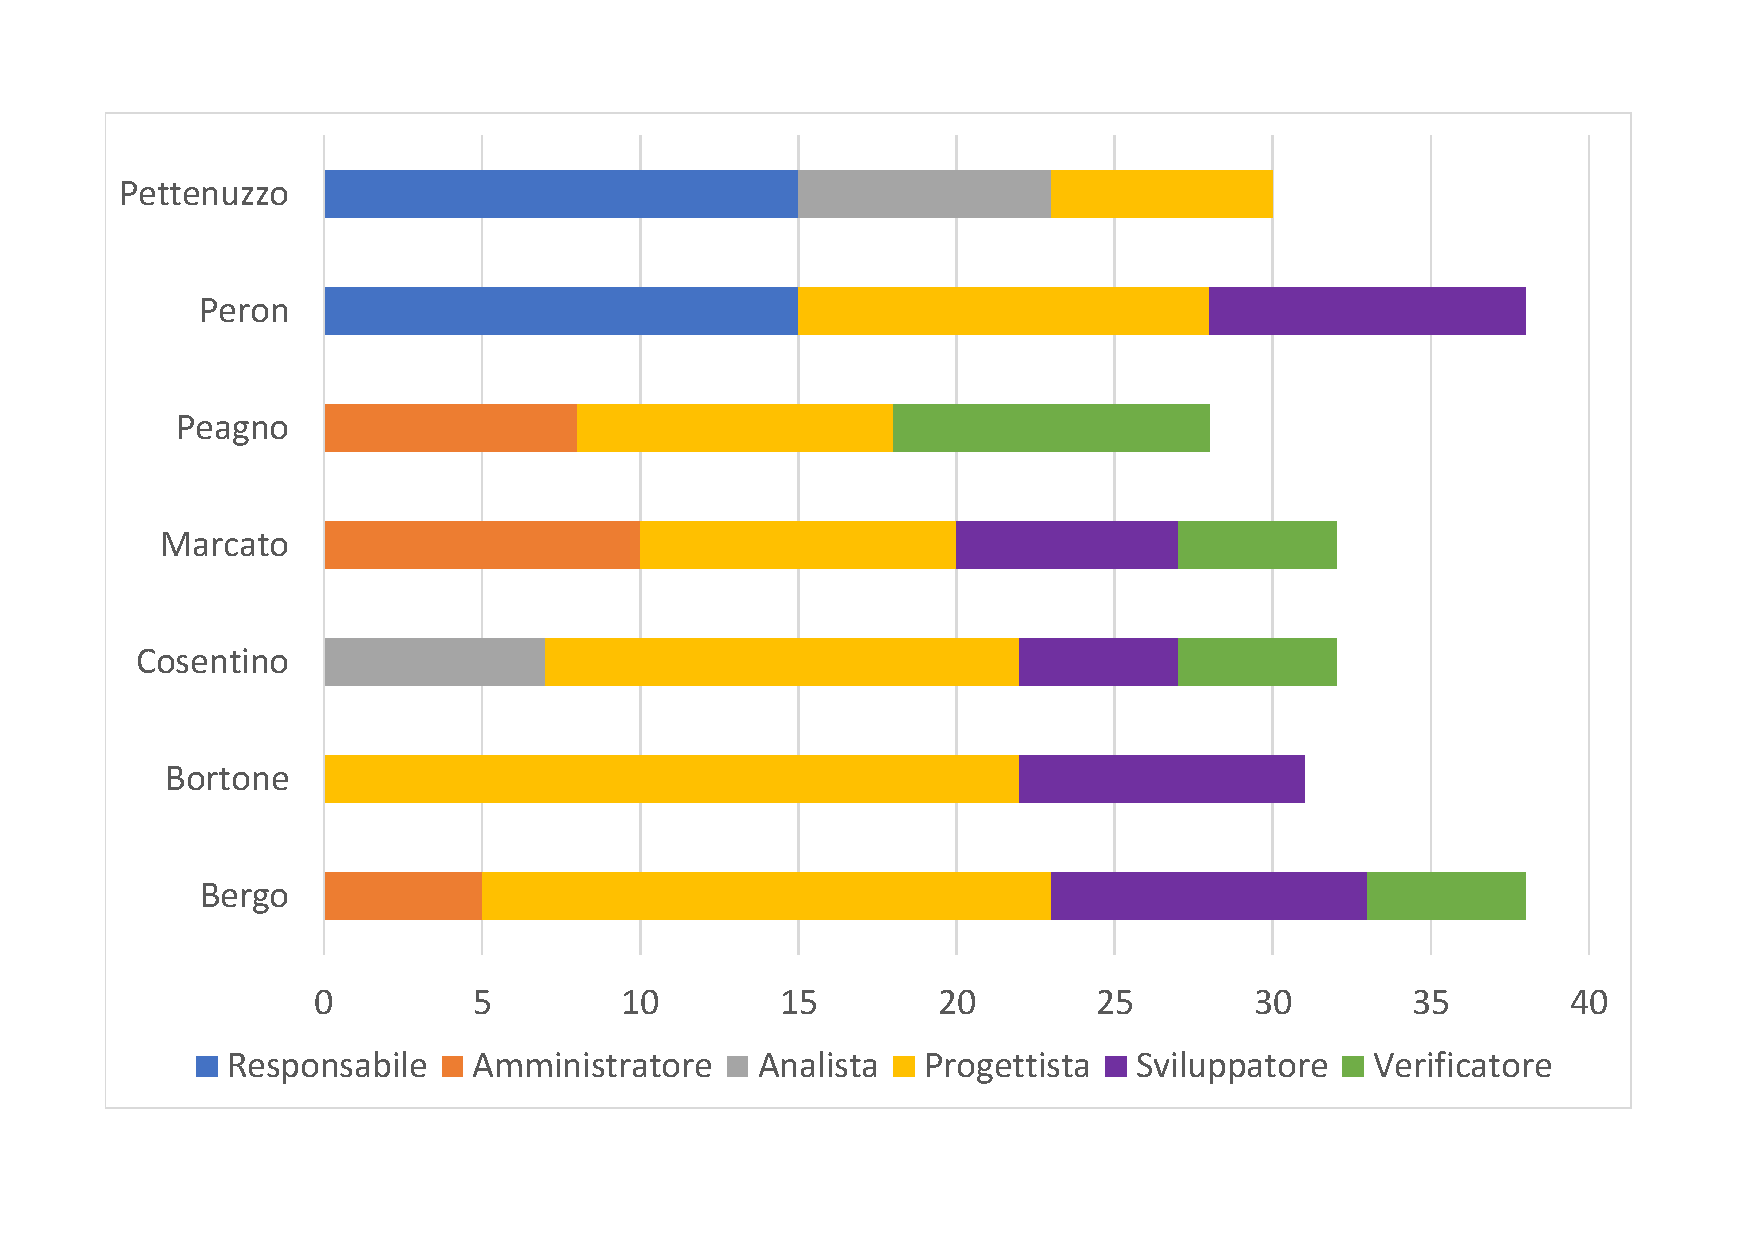
\includegraphics[scale=0.45]{images/consuntivoRP.pdf}
		\caption{Istogramma del consuntivo della fase 2}
	\end{figure}
	
	\subsubsection{Costo}
	Le seguenti tabelle indicano i costi della fase 2. Nell'ultima colonna vengono indicate le differenze tra costi previsti e costi effettivi ($previsto - effettivo$): valori positivi indicano i risparmi e valori negativi indicano le perdite.
		
	\begin{table}[H]
		\centering
		\begin{tabular}{| l | l | l |}
			\rowcolor{LightBlue}
			\textbf{\color{white}Membro}
			& \textbf{\color{white}Costo}
			& \textbf{\color{white}Differenza}\\
			Bergo		& 721€	& 9€\\
			Bortone		& 619€	& 53€\\
			Cosentino	& 655€	& -94€\\
			Marcato		& 600€	& 0€\\
			Peagno		& 530€	& 52€\\
			Peron		& 886€	& -66€\\
			Pettenuzzo	& 804€	& 6€\\ \hline
			\textbf{Totale} & 4815	& -40€\\ \hline
		\end{tabular}
		\caption{Costo effettivo di ciascun membro nella fase 2}	
	\end{table}
	
	\begin{table}[H]
		\centering
		\begin{tabular}{| l | l |l|}
			\rowcolor{LightBlue}
			\textbf{\color{white}Membro}
			& \textbf{\color{white}Costo}
			& \textbf{\color{white}Differenza}\\

			Responsabile	& 900€	& 0€\\
			Amministratore 	& 460€ 	& -80€\\
			Analista 		& 375€ 	& 0€\\
			Progettista 	& 2090€	& -110€\\
			Programmatore 	& 615€	& 150€\\
			Verificatore 	& 375€	& 0€\\ \hline
			\textbf{Totale} & 4815€	& -40€\\ \hline
		\end{tabular}
		\caption{Costo effettivo di ciascun ruolo nella fase 2}
	\end{table}
	
	\subsubsection{Conclusioni}
		\paragraph{Costi\\}
La cifra prevista per l'investimento era di \textbf{4775€}, il costo effettivo si è rivelato con un aumento di \textbf{40€} rispetto alla stima iniziale. Per cui la cifra alla fine della fase 2 corrisponde a \textbf{4815€}.
 		
		\paragraph{Scostamenti\\}
Il gruppo ha riscontrato delle difficoltà nella progettazione del Proof of Concept, la quale ha richiesto più ore rispetto a quanto preventivato. Le difficoltà derivano da una scelta tecnologica che si è rivelata errata per questo motivo sono state prese come alternativa tecnologie già conosciute dai componenti. In questo modo le ore di codifica sono state rispettate in modo soddisfacente senza grandi imprevisti.
\newpage
\subsection{Fase 3 (2019-03-16 - 2019-04-19)}
	\subsubsection{Ore impiegate}
	La seguente tabella indica le ore impiegate durante la fase 3. Tra parentesi viene indicata la differenza tra ore preventivate e ore impiegate ($preventivo - consuntivo$): valori positivi indicano le ore risparmiate e valori negativi indicano le ore in eccesso.
	
	\begin{table}[H]
		\centering
		\begin{tabular}{| l | c c c c c c | c |}
			\rowcolor{LightBlue}
			& \multicolumn{7}{c}{\textbf{\color{white}Numero di ore}}	\\
			
			\rowcolor{LightBlue}
			\textbf{\color{white}Membro}
			& \textbf{\color{white}RES}
			& \textbf{\color{white}AMM}
			& \textbf{\color{white}AN}
			& \textbf{\color{white}PRO}
			& \textbf{\color{white}DEV}
			& \textbf{\color{white}VER}
			& \textbf{\color{white}Totali}\\
			Bergo     		& 15  (0) & 2 (+2) 	& -  (0) 		& 8 (-2) & 10 (0) & 10 (0) 	& 45(0)\\
			Bortone   		& 11  (-4) & -  (0) 	& -  (-5) 		& 8 (0) & 16 (+9) & 12 (+2)	& 47(+2)\\
			Cosentino & - (0) & 5 (0) 	& 2 (+2) & 21 (0) & 18 (-3) & - (0)	& 46(-1)\\
			Marcato  & -  (0) & 5 (+5) 	& -  (0) & 15 (-10) & 26 (+1) & - (0) & 46(-4)\\
			Peagno    		& -  (0) & - (0) & -  (0) & 20 (-5) & 27 (+2) & - (0)	& 47(-3)\\
			Peron   & -  (0) & -  (0) 	& -  (0) & 15 (0) & 20 (+5) &  10 (-5)	& 45(0)\\
			Pettenuzzo 		& - (0) & 5 (+5) & 3 (-2) & 8 (-2) & 26 (+1) & 10 (0)	& 52(+2)\\ \hline
		\end{tabular}
		\caption{Ore di lavoro impiegate per membro/ruolo della fase 3}
		
		\begin{figure}[H]
			\centering
			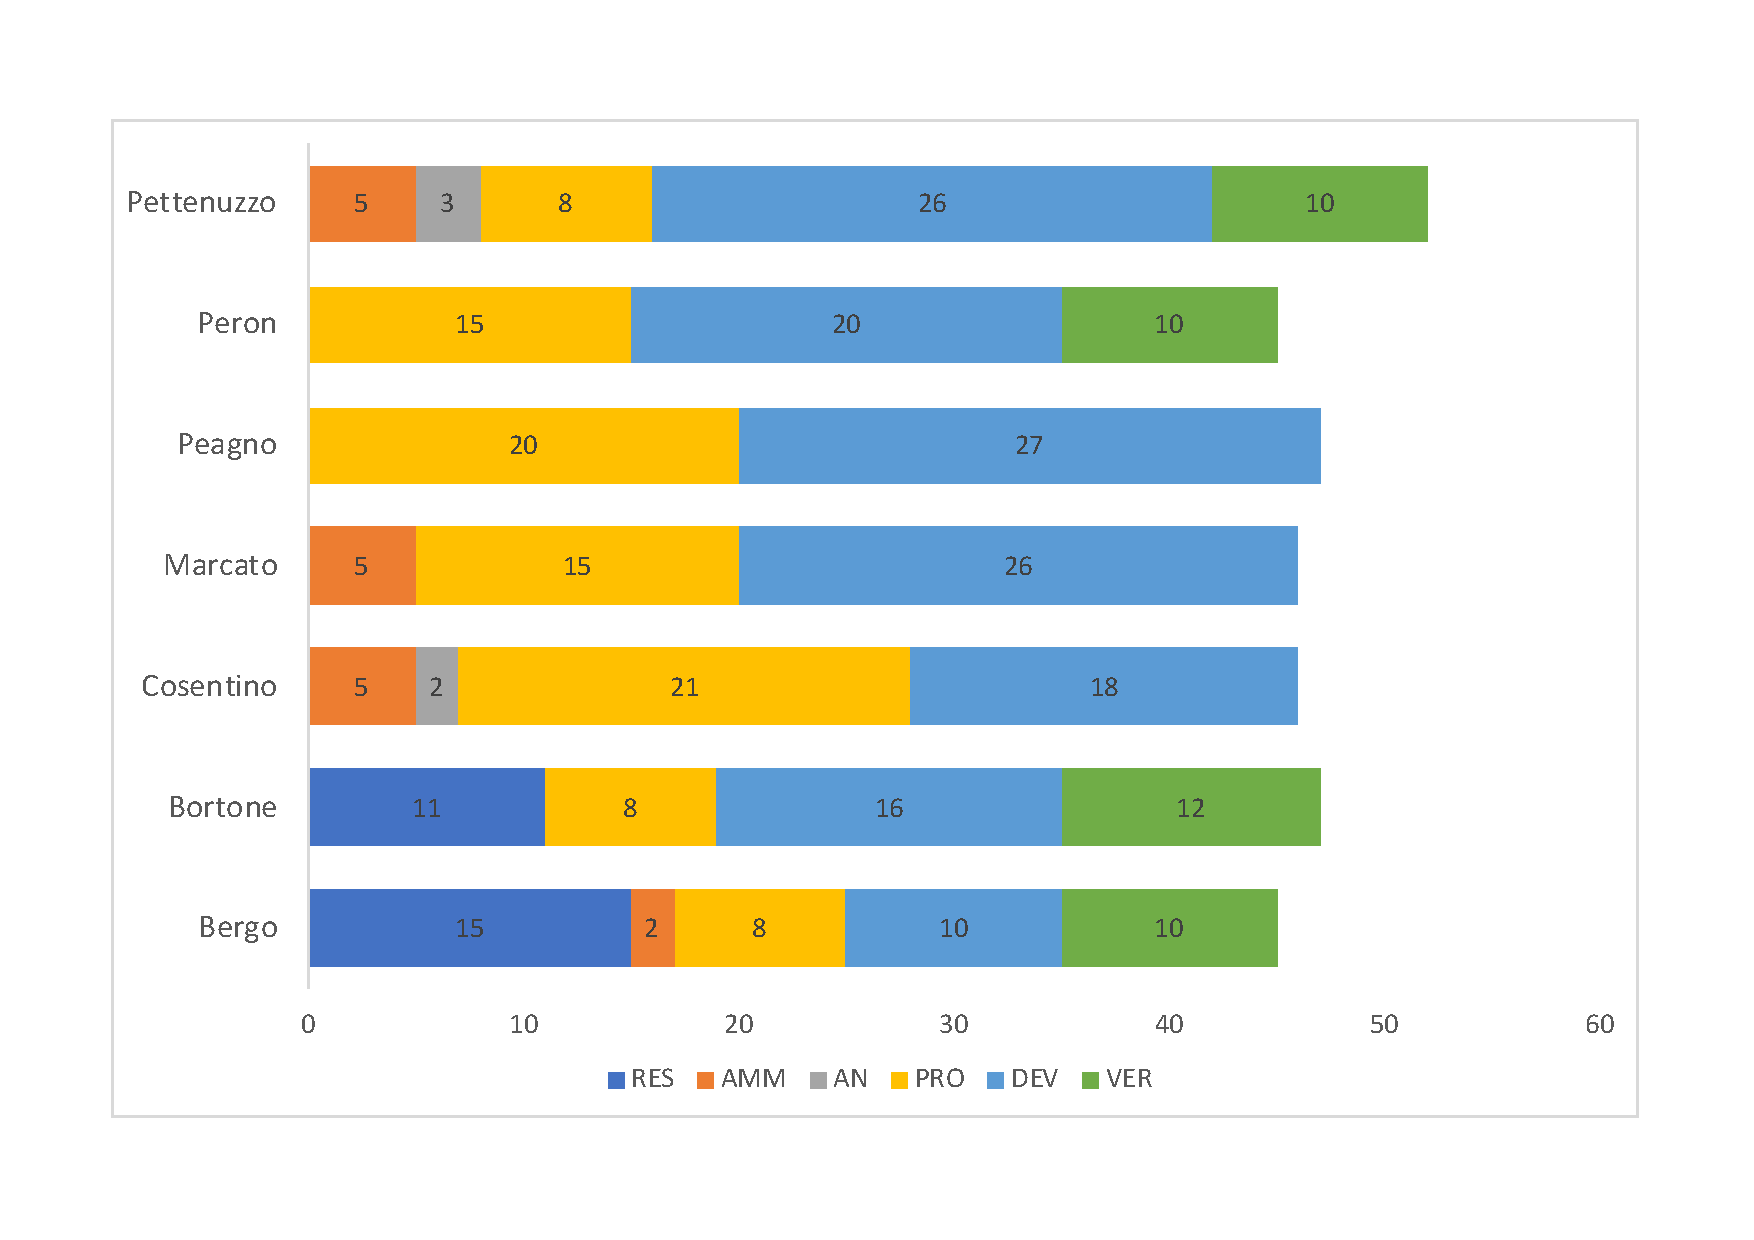
\includegraphics[scale=0.45]{images/consuntivoRQ.pdf}
			\caption{Istogramma del consuntivo della fase 3}
		\end{figure}
		
		
	\end{table}
	\subsubsection{Costo}
		Le seguenti tabelle indicano i costi della fase 3. Nell'ultima colonna vengono indicate le differenze tra costi previsti e costi effettivi ($previsto - effettivo$): valori positivi indicano i risparmi e valori negativi indicano le perdite.
		
		\begin{table}[H]
			\centering
			\begin{tabular}{| l | l | l |}
				\rowcolor{LightBlue}
				\textbf{\color{white}Membro}
				& \textbf{\color{white}Costo}
				& \textbf{\color{white}Differenza}\\
				Bergo		& 966€	& 4€\\
				Bortone		& 926€	& 80€\\
				Cosentino	& 882€	& -5€\\
				Marcato		& 820€	& 105€\\
				Peagno		& 845€	& 80€\\
				Peron		& 780€	& 0€\\
				Pettenuzzo	& 891€	& -21€\\ \hline
				\textbf{Totale} & 6110	& 243€\\ \hline
			\end{tabular}
			\caption{Costo effettivo di ciascun membro nella fase 3}	
		\end{table}
	
	
	\begin{table}[H]
		\centering
		\begin{tabular}{| l | l |l|}
			\rowcolor{LightBlue}
			\textbf{\color{white}Membro}
			& \textbf{\color{white}Costo}
			& \textbf{\color{white}Differenza}\\
			
			Responsabile	& 780€	& 120€\\
			Amministratore 	& 340€ 	& -240€\\
			Analista 		& 125€ 	& 125€\\
			Progettista 	& 2090€	& 418€\\
			Programmatore 	& 2145€	& -225€\\
			Verificatore 	& 630€	& 45€\\ \hline
			\textbf{Totale} & 6110€	& 243€\\ \hline
		\end{tabular}
		\caption{Costo effettivo di ciascun ruolo nella fase 3}
	\end{table}


	\subsubsection{Gestione dei rischi}
	Durante lo svolgersi di questa fase, nessuno dei rischi elencati in \S2 si è verificato. Abbiamo provveduto ad abbassare la probabilità o pericolo dei seguenti rischi: 
	\begin{itemize}
	\item 		O01 Superamento dei costi: dato che il progetto è in una fase avanzata, è più semplice pianificare e conseguentemente più facile rientrare nei costi;
	\item 		G03 Problemi di comunicazione: il team è riuscito a comunicare in maniera più tempestiva;
	\item		T01 Tecnologie da applicare: le tecnologie applicate in questa fase sono già ben comprese dal team;
	\item 		G02 Contrasti nel team: ormai il team si conosce, mostrando certe affinità caratteriali ed il rischio è quasi nullo.
	\end{itemize}

	\subsubsection{Conclusioni}
	\paragraph{Costi\\}\noindent\\
 La cifra prevista per l'investimento era di \textbf{6353€}, il costo effettivo è diminuito rispetto alla stima iniziale. Per cui la cifra alla fine della fase 3 è di \textbf{6110€}.Tenendo conto dell'aumento di \textbf{40€} della fase precedente il costo effettivo è \textbf{6150€}.
I rimasti \textbf{203€} saranno reinvestiti nella successiva fase.

\paragraph{Scostamenti\\}\noindent\\
La pianificazione della fase 4 è stata modificata in base a questo consuntivo.
Il gruppo è in ritardo nei requisiti, infatti sono stati spostati nell 'incremento 1 della fase 4. Il numero di ore rispetto a quanto preventivato sono di 4 in meno perchè l'intervento del responsabile non era necessario in quanto abbiamo speso più tempo nella fase di codifica.
	\newpage
	\subsection{Preventivo a finire}
La seguente tabella presenta l'attuale preventivo a finire. Se il valore del consuntivo di un determinato periodo non è ancora presente, per il conteggio totale verrà utilizzato il valore del preventivo.

\begin{table}[H]
			\centering
		\begin{tabular}{| l | l | l | l |}
			\rowcolor{LightBlue}
			\textbf{\color{white}Fase}
			& \textbf{\color{white}Preventivo}
			& \textbf{\color{white}Consuntivo}
			& \textbf{\color{white}Variazione}
			\\
			
			Fase 2 			& 4775€ 	& 4815€ & -40€\\
			Fase 3 		& 6353€ 	& 6110 & +243\\
			Fase 4			& 3037€ 	& - & -\\
			\textbf{Totale} & 14090€ & 13962€ & +203€\\ \hline
		\end{tabular}
		\caption{Preventivo a finire aggiornato al termine della fase 3}	
\end{table}


\newpage
\subsection{Fase 4 (2019-04-20 - 2019-05-17)}
	\subsubsection{Ore impiegate}
	La seguente tabella indica le ore impiegate durante la fase 4. Tra parentesi viene indicata la differenza tra ore preventivate e ore impiegate ($preventivo - consuntivo$): valori positivi indicano le ore risparmiate e valori negativi indicano le ore in eccesso.
	
	\begin{table}[H]
		\centering
		\begin{tabular}{| l | c c c c c c | c |}
			\rowcolor{LightBlue}
			& \multicolumn{7}{c}{\textbf{\color{white}Numero di ore}}	\\
			
			\rowcolor{LightBlue}
			\textbf{\color{white}Membro}
			& \textbf{\color{white}RES}
			& \textbf{\color{white}AMM}
			& \textbf{\color{white}AN}
			& \textbf{\color{white}PRO}
			& \textbf{\color{white}DEV}
			& \textbf{\color{white}VER}
			& \textbf{\color{white}Totali}\\
			Bergo & -(0) & -(0) & -(0) & 11(-4) & 11(+1) & -(0) & 22(-3)\\
			Bortone & -(0) & -(0) & -(0) & 8(0) & 9(+3) & 10(-4) & 27(-1)\\
			Cosentino & -(0) & 3(+2) & -(0) & 7(0) & 7(-1) & 10(-4) & 27(-3)\\
			Marcato  & -(0) & 0(-5) & -(0) & 0(-7) & 16(-9) & 11(-6) & 27(-3)\\
			Peagno & 10(0) & 0(-4) & -(0) & 0(-2) & 16(-9) & 11(-4) & 30(0)\\
			Peron   & -(0) & 0(-2) & -(0) & 5(-1) & 9(-1) &  8(-2)	& 22(0)\\
			Pettenuzzo & 0(-11) & -(0) & -(0) & 15(-10) & -(0) & 8(-3) & 23(-2)\\ \hline
		\end{tabular}
		\caption{Ore di lavoro impiegate per membro/ruolo della fase 4}
		
		\begin{figure}[H]
			\centering
			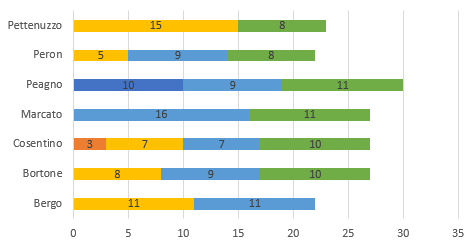
\includegraphics[scale=1]{images/consuntivoRA.png}
			\caption{Istogramma del consuntivo della fase 4}
		\end{figure}
	\end{table}
	
	\subsubsection{Costo}
		Le seguenti tabelle indicano i costi della fase 4. Nell'ultima colonna vengono indicate le differenze tra costi previsti e costi effettivi ($previsto - effettivo$): valori positivi indicano i risparmi e valori negativi indicano le perdite.
		
		\begin{table}[H]
			\centering
			\begin{tabular}{| l | l | l |}
				\rowcolor{LightBlue}
				\textbf{\color{white}Membro}
				& \textbf{\color{white}Costo}
				& \textbf{\color{white}Differenza}\\
				Bergo		& 407€	& -73€\\
				Bortone		& 461€	& -15€\\
				Cosentino	& 469€	& -35€\\
				Marcato		& 405€	& 29€\\
				Peagno		& 600€	& 34€\\
				Peron		& 365€	& 3€\\
				Pettenuzzo	& 450€	& 65€\\ \hline
				\textbf{Totale} & 3157	& 8€\\ \hline
			\end{tabular}
			\caption{Costo effettivo di ciascun membro nella fase 4}	
		\end{table}
		
			
	\begin{table}[H]
		\centering
		\begin{tabular}{| l | l |l|}
			\rowcolor{LightBlue}
			\textbf{\color{white}Membro}
			& \textbf{\color{white}Costo}
			& \textbf{\color{white}Differenza}\\
			
			Responsabile	& 300€	& 330€\\
			Amministratore 	& 260€ 	& 260€\\
			Analista 		& 0€ 	& 0€\\
			Progettista 	& 1012€	& -132€\\
			Programmatore 	& 915€	& -105€\\
			Verificatore 	& 870€	& -345€\\ \hline
			\textbf{Totale} & 3157€	& 8€\\ \hline
		\end{tabular}
		\caption{Costo effettivo di ciascun ruolo nella fase 4}
	\end{table}